% =====================================================================
%  A1 PORTRAIT POSTER TEMPLATE (594 x 841 mm)
%  Topic: RGB-D topological mapping / two-layer GNG for the ceiling robot
%
%  This is a BIG-FONT / BULLET-POINT variant of poster_rgbd_topo_A1.tex:
%  - the supervisor/author line under the title is larger
%  - prose paragraphs are trimmed to bullet points instead of full sentences
%  Keep the base poster_rgbd_topo_A1.tex untouched; edit this file instead.
%
%  This is a CLONE of docs/poster_A1_energy_aware/poster_energy_aware_A1.tex:
%  identical layout, colours and macros, but the content is a skeleton.
%
%  >>> HOW TO USE <<<
%   1. Everything wrapped in \TODO{...} is a placeholder -- it prints in RED
%      so an unfinished poster is obvious. Replace, do not just delete the
%      macro, or the surrounding sentence may stop making sense.
%   2. \FIGBOX{<height>}{<caption>} is a grey placeholder frame. Swap it for
%      \IG{<width fraction>}{<file in figure/>} once the real asset exists.
%   3. NEVER type a number you have not measured. Leave it as \TODO{}.
%   4. Section text below is drawn from the reachability_gng README (method,
%      not results), so the *how it works* parts are already accurate.
%
%  Build:  pdflatex poster_rgbd_topo_A1.tex
%
%  Tuning knobs (preamble): \bodysize / \bodyskip for all body text,
%  \pillsize for section headers, \figscale scales every \IG figure.
% =====================================================================
\documentclass[20pt,a4paper]{extarticle}

\usepackage[
  paperwidth=594mm, paperheight=841mm,
  left=14mm, right=14mm, top=13mm, bottom=13mm
]{geometry}

\usepackage[T1]{fontenc}
\usepackage[utf8]{inputenc}
\usepackage[scaled=0.98]{helvet}
\renewcommand{\familydefault}{\sfdefault}

\usepackage{amsmath,amssymb}
\usepackage{graphicx}
\usepackage{xcolor}
\usepackage[most]{tcolorbox}
\usepackage{tikz}
\usetikzlibrary{positioning,calc,arrows.meta}
\usepackage{eso-pic}
\usepackage{enumitem}
\usepackage{booktabs}
\usepackage{array}
\usepackage{ragged2e}
\usepackage{anyfontsize}

\graphicspath{{figure/}}

% ------------------------------------------------------------- knobs
\newcommand{\bodysize}{21}
\newcommand{\bodyskip}{25.5}
\newcommand{\pillsize}{28}
\def\figscale{0.92}
\newcommand{\IG}[2]{\includegraphics[width=\figscale\dimexpr#1\linewidth\relax]{#2}}

% ---------------------------------------------------------------- colors
\definecolor{pgold}{HTML}{F5B335}
\definecolor{pgoldd}{HTML}{D98C0F}
\definecolor{pbody}{HTML}{1A1A1A}
\definecolor{pblue}{HTML}{1F4E79}
\definecolor{pgrey}{HTML}{6E6E6E}

\color{pbody}
\setlength{\parindent}{0pt}
\setlength{\parskip}{1pt}
\renewcommand{\arraystretch}{1.12}

% ------------------------------------------------- outer rounded frame
\AddToShipoutPictureBG{%
  \begin{tikzpicture}[remember picture, overlay]
    \draw[pgold, line width=3.2pt, rounded corners=16pt]
      ($(current page.south west)+(8mm,8mm)$)
      rectangle
      ($(current page.north east)+(-8mm,-8mm)$);
  \end{tikzpicture}%
}

% ------------------------------------------------------ section pill
\newtcolorbox{sectionpill}{
  enhanced, width=\linewidth,
  colback=pgold, colframe=pgold,
  arc=8mm, boxrule=0pt,
  left=4mm, right=4mm, top=1.2mm, bottom=1.2mm,
  halign=flush center, valign=center,
  before skip=3.5mm, after skip=1.8mm
}
\newcommand{\psection}[1]{%
  \begin{sectionpill}\bfseries\fontsize{\pillsize}{\pillsize}\selectfont #1\end{sectionpill}}

% ------------------------------------------------------ highlight box
\newtcolorbox{keybox}{
  enhanced, width=\linewidth,
  colback=pgold!16!white, colframe=pgold,
  arc=4mm, boxrule=1.4pt,
  left=4mm, right=4mm, top=1.8mm, bottom=1.8mm,
  before skip=2mm, after skip=2mm
}

% ------------------------------------------------------ list styles
\setlist[itemize,1]{leftmargin=6mm, itemindent=0mm, topsep=1pt, itemsep=2pt,
                    parsep=0pt, label=\small\textcolor{pgoldd}{$\bullet$}}
\setlist[itemize,2]{leftmargin=6mm, itemindent=0mm, topsep=1pt, itemsep=1pt,
                    parsep=0pt, label=\small\textcolor{pgoldd}{$\circ$}}

% ------------------------------------------------------ helpers
\newcommand{\figcap}[1]{{\par\vspace{0.8mm}\centering
  \fontsize{18}{21}\selectfont\itshape\color{pgrey}#1\par\vspace{0.8mm}}}
\newcommand{\num}[1]{\textcolor{pblue}{\bfseries #1}}
\newcommand{\lead}[1]{\textbf{#1}}

% -------------------------------------------- placeholders (REMOVE LATER)
\newcommand{\TODO}[1]{\textcolor{red}{\bfseries[TODO: #1]}}
\newcommand{\FIGBOX}[2]{%
  \begin{center}
  \begin{tcolorbox}[enhanced, width=\linewidth, height=#1,
    colback=pgrey!8!white, colframe=pgrey!45!white, boxrule=1.2pt,
    arc=3mm, halign=center, valign=center, before skip=2mm, after skip=1mm]
    {\fontsize{16}{19}\selectfont\color{pgrey}\itshape figure placeholder\\[1mm]#2}
  \end{tcolorbox}
  \end{center}}

\pagestyle{empty}

\begin{document}
\fontsize{\bodysize}{\bodyskip}\selectfont

% =====================================================================
%  HEADER
% =====================================================================
\begin{tcolorbox}[enhanced, width=\linewidth,
  colback=white, colframe=pgold, arc=10mm, boxrule=2.6pt,
  left=6mm, right=6mm, top=2mm, bottom=2mm]
\begin{minipage}[c]{0.085\linewidth}
  \centering
  \bfseries\fontsize{38}{38}\selectfont P-XX
\end{minipage}%
\begin{minipage}[c]{0.79\linewidth}
  \centering
  {\bfseries\fontsize{20}{23}\selectfont
   2026 The Term-End Evaluation, Department of Mechanical Systems Engineering, TMU.\par}
  \vspace{2mm}
  {\bfseries\fontsize{40}{46}\selectfont
   Two-Layer Topological Mapping for\\
   Energy-Aware Arm and Base Selection\\
   on a Dual-Gantry Quad-Arm Ceiling Robot\par}
  \vspace{2.5mm}
  {\bfseries\fontsize{30}{34}\selectfont
   Naoyuki Kubota Laboratory, D1, Raditya Artha Rochmanto\par}
  {\fontsize{24}{28}\selectfont
   email: rochmanto-artha@ed.tmu.ac.jp\par}
\end{minipage}%
\begin{minipage}[c]{0.125\linewidth}
  \centering
  
\includegraphics[width=1\linewidth]{tmu_logo.jpg}\\[1.5mm]
  {\bfseries\fontsize{16}{18}\selectfont\color{pgrey} CONFIDENTIAL}
\end{minipage}
\end{tcolorbox}

% ------------------------------------------------------------- tagline
\begin{center}
  \bfseries\fontsize{27}{31}\selectfont
  One topological representation, two layers:\\
  the room the robot sees, and the reach each arm owns, priced in energy.
\end{center}

\vspace{-1mm}

% =====================================================================
%  TWO COLUMNS
% =====================================================================
\noindent
\begin{minipage}[t]{0.487\linewidth}
% ================================================= LEFT COLUMN =======
\fontsize{22.5}{27}\selectfont

\psection{Background}

\begin{minipage}[c]{0.27\linewidth}
  \centering
  \IG{1.0}{ceilingarm_tll-edit.jpg}
\end{minipage}\hfill
\begin{minipage}[c]{0.70\linewidth}
  \RaggedRight
  \begin{itemize}
    \item Aging population $\rightarrow$ assistive robots \textbf{in-home}
    \item Small, cluttered, \textbf{shared with residents}
    \item \textbf{Ceiling-mounted} $\rightarrow$ floor stays free
    \item \textbf{2 rails $\times$ 2 arms} = 4 arms, \textbf{8-DOF} each
    \item \textbf{RGB-D only}, no LIDAR
  \end{itemize}
\end{minipage}

\psection{Problems}

\begin{itemize}
  \item \lead{P1:} which arm, where the base stops --- coupled
  \item \lead{P2:} fixed-base maps only, reachable / not
  \item \lead{P3:} occupancy has no topology
\end{itemize}

\psection{Core Idea: One GNG, Two Layers}

\begin{keybox}
\textbf{One Growing Neural Gas}, fitted twice: what the cameras see
(environment) and what each arm can reach (capability).
\end{keybox}

\psection{Layer 1: Environment GNG from RGB-D}

\begin{itemize}
  \item 2 overhead RGB-D cameras, \textbf{no LIDAR}
  \item \lead{Placement:} ceiling-mounted ($z\approx2.05$~m), diagonally
        opposite corners, angled down/inward at the table
  \item \texttt{depth\_cloud}: depth $\rightarrow$ world points, no seg.\ gate
  \item GNG on the cloud $\rightarrow$ scene \emph{topology}
  \item \lead{Static:} frozen once. \lead{Dynamic:} live remainder only
  \item Union $\rightarrow$ MoveIt~2 planning scene; tracks by Hungarian match
\end{itemize}

\vspace{1mm}
{\centering
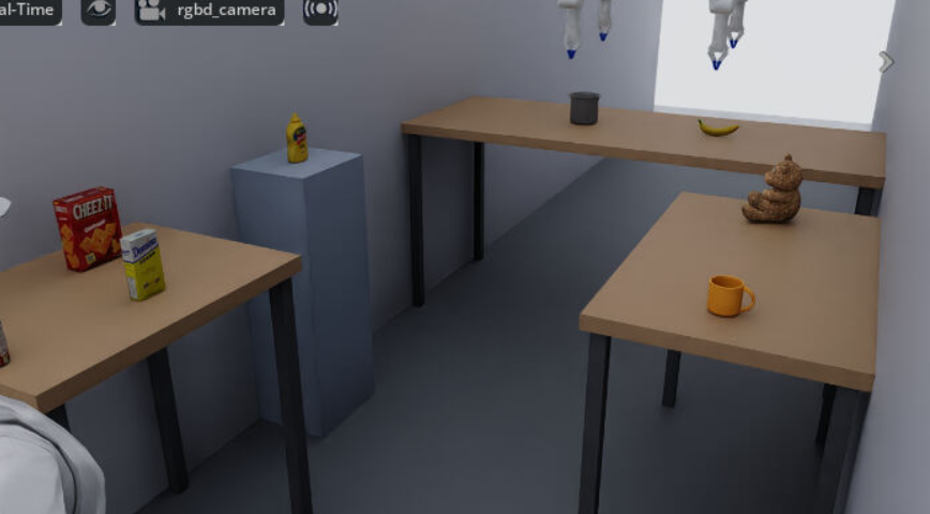
\includegraphics[trim=0 0 0 34, clip, width=0.487\linewidth]{view_rgbd1.png}\hfill
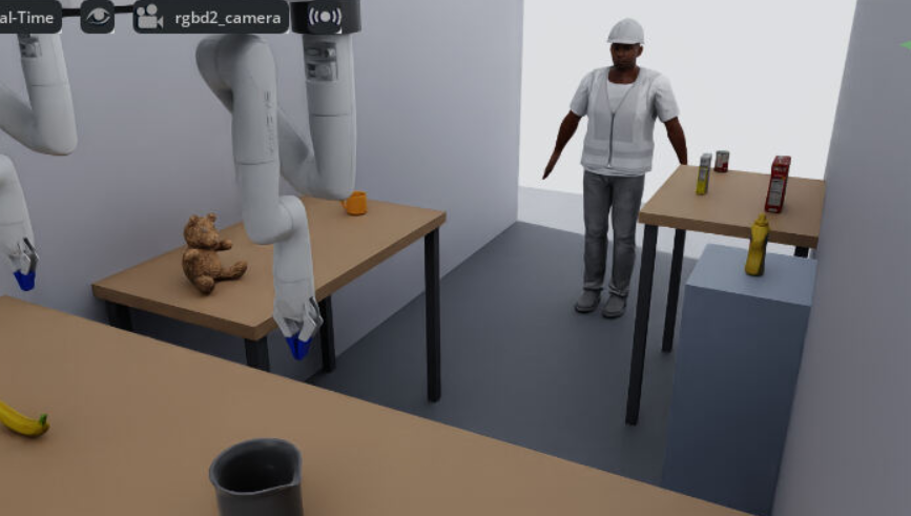
\includegraphics[trim=0 0 0 36, clip, width=0.487\linewidth]{view_rgbd2.png}\par}
\figcap{The two overhead RGB-D views: the entire input (\textbf{NVIDIA Isaac Sim}).}

\vspace{1.5mm}
{\centering
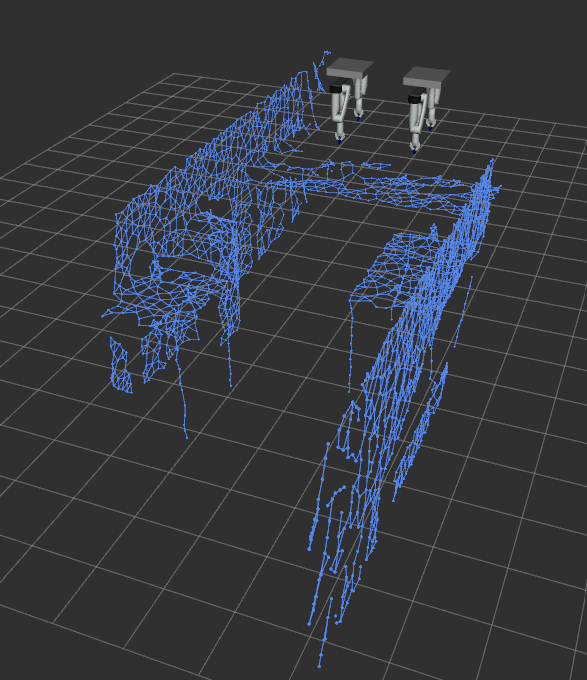
\includegraphics[height=78mm]{GNG_static3.png}\hspace{5mm}
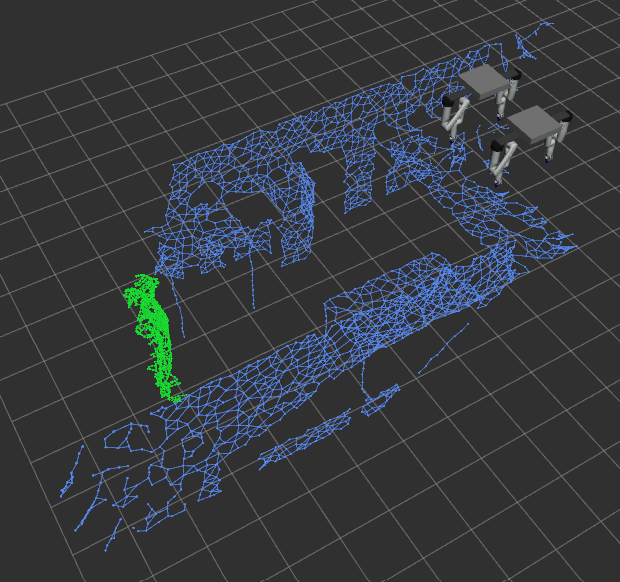
\includegraphics[height=78mm]{GNG_dynamic3.png}\par}
\figcap{Left: frozen \textcolor{blue!70!black}{static} backbone. Right: plus
\textcolor{green!45!black}{dynamic} remainder (a person).}

\begin{keybox}
\lead{Static vs.\ dynamic budget:} \num{1800}-node static backbone
(offline, multi-epoch, captured once) vs.\ \num{800}-node live cap
(online, single pass per frame) --- same GNG, different node budget
\& training regime per layer.
\end{keybox}

\psection{Layer 2: Base-Aware Capability GNG}

\begin{itemize}
  \item Sample \textbf{full 8-DOF} $\mathbf{q}$, FK (Pinocchio),
        manipulability $w=\sqrt{\det(JJ^{\!\top})}$
  \item Node stores $[\,\mathbf{x}\mid\mathbf{q}\,]$: point + config,
        \textbf{rail included}
  \item \textbf{Boundary seeding} $\rightarrow$ 4 maps (one per arm)
\end{itemize}

\vspace{1mm}
{\centering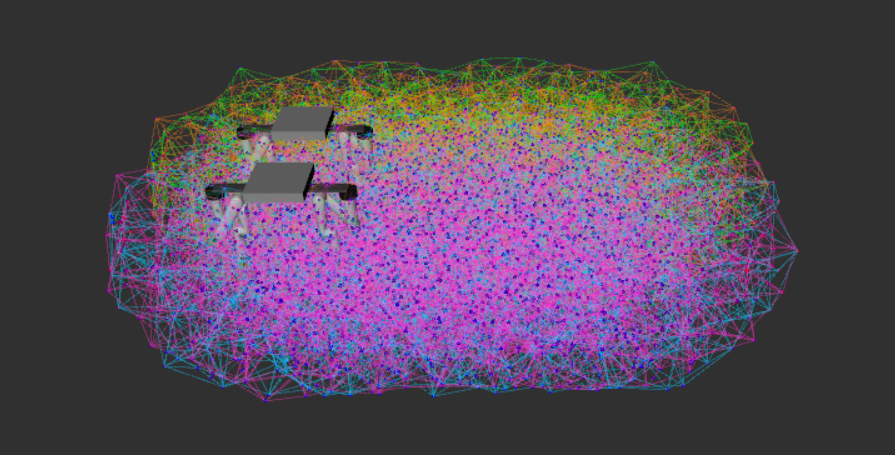
\includegraphics[trim=95 45 90 45, clip,
   width=\figscale\dimexpr0.78\linewidth\relax]{gng_capability.png}\par}
\figcap{Capability layer of one arm (RViz), coloured by manipulability.}

\begin{keybox}
\lead{Per arm:} 80{,}000 FK samples $\rightarrow$ \num{2915 nodes}
(600 boundary), 14{,}547 edges, spacing \num{0.090~m}.
\end{keybox}

\end{minipage}\hfill
% ================================================= RIGHT COLUMN ======
\begin{minipage}[t]{0.487\linewidth}

\psection{System and Pipeline}

{\centering
\resizebox{\linewidth}{!}{%
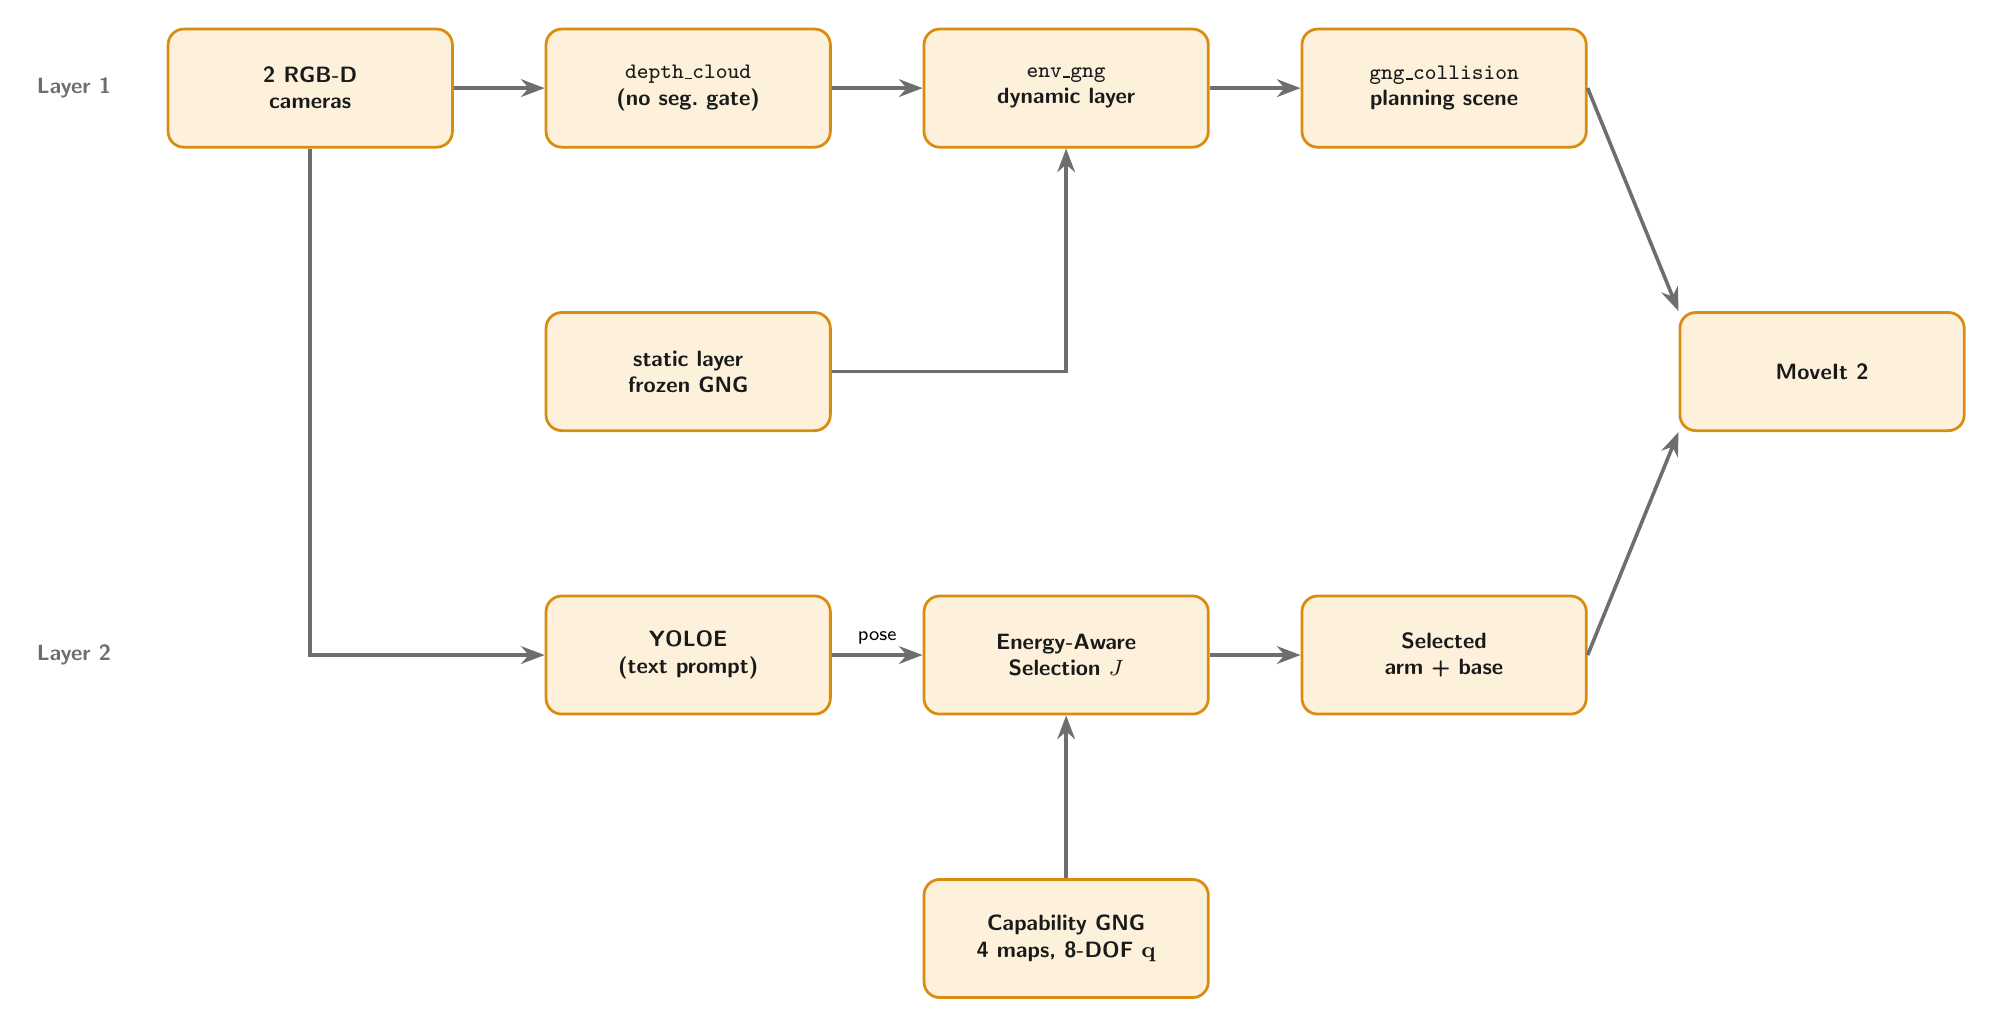
\begin{tikzpicture}[>=Stealth, thick, font=\footnotesize,
  box/.style={draw=pgoldd, line width=1pt, fill=pgold!18!white, text=pbody,
              rounded corners=2mm, align=center, minimum height=15mm,
              text width=34mm, inner sep=3pt, font=\bfseries\footnotesize},
  lay/.style={font=\bfseries\footnotesize, text=pgrey},
  arr/.style={-{Stealth[length=3mm]}, line width=1.3pt, draw=pgrey}]
  % --- geometry path (top row): Layer 1
  \node[box] (cam)  at (0,0)      {2 RGB-D\\cameras};
  \node[box] (dc)   at (4.8,0)    {\texttt{depth\_cloud}\\(no seg.\ gate)};
  \node[box] (env)  at (9.6,0)    {\texttt{env\_gng}\\dynamic layer};
  \node[box] (col)  at (14.4,0)   {\texttt{gng\_collision}\\planning scene};
  \node[box] (stat) at (4.8,-3.6) {static layer\\frozen GNG};
  % --- identity + decision path (bottom row): Layer 2
  \node[box] (seg)  at (4.8,-7.2) {YOLOE\\(text prompt)};
  \node[box] (sel)  at (9.6,-7.2) {Energy-Aware\\Selection $J$};
  \node[box] (cap)  at (9.6,-10.8){Capability GNG\\4 maps, 8-DOF $\mathbf{q}$};
  \node[box] (arm)  at (14.4,-7.2){Selected\\arm + base};
  \node[box] (mv)   at (19.2,-3.6){MoveIt~2};
  \node[lay, anchor=east] at (-2.4,0)     {Layer 1};
  \node[lay, anchor=east] at (-2.4,-7.2)  {Layer 2};
  \draw[arr] (cam)  -- (dc);
  \draw[arr] (dc)   -- (env);
  \draw[arr] (env)  -- (col);
  \draw[arr] (stat) -| (env);
  \draw[arr] (cam.south) |- (seg.west);
  \draw[arr] (seg)  -- node[above, font=\scriptsize] {pose} (sel);
  \draw[arr] (cap)  -- (sel);
  \draw[arr] (sel)  -- (arm);
  \draw[arr] (col.east) -- (mv.north west);
  \draw[arr] (arm.east) -- (mv.south west);
\end{tikzpicture}}\par}
\figcap{Layer 1 (geometry) is decoupled from Layer 2 (identity + decision).}

\psection{Energy-Aware Selection Cost $J$}

\begin{keybox}
\centering
$\displaystyle
J = w_{gl}\frac{\Delta_{lin}}{\rho_{gl}}
  + w_{gr}\frac{\Delta_{rot}}{\rho_{gr}}
  + w_{arm}\frac{\Delta_{arm}}{\rho_{arm}}
  + w_{dist}\frac{e}{\rho_{dist}}
  - w_{manip}\frac{m}{\rho_{manip}}$
\end{keybox}

\begin{itemize}
  \item Rail/arm travel, tool distance, manipulability ---
        \textbf{fit by OLS} on 168 picks ($R^2=0.857$): rail dominates
  \item \lead{GNG $\rightarrow$ $J$:} every \textbf{capability-layer node}
        near the target (all 4 arms) scored by $J$ from its own $\mathbf{q}$
  \item \lead{Selection:} \textbf{lowest-$J$ first}, \textbf{plan-only};
        first collision-free plan wins
\end{itemize}

\psection{Experiments and Results}

\begin{itemize}
  \item \lead{Feasibility, not just efficiency:} \num{93.3\%} multi-arm
        success vs.\ \num{63--65\%} for any single fixed arm
  \item \lead{Why:} rail active $\rightarrow$ \textbf{$4\times$}
        reachable volume (\num{1.9$\rightarrow$7.9~m$^3$})
  \item \lead{Boundary seeding:} reach-surface error \num{0.221~m
        $\rightarrow$ 0.008~m}
\end{itemize}

\vspace{1mm}
{\centering\IG{1.0}{results.pdf}\par}
\figcap{(a) Reachable volume. (b) Trajectory energy per policy ($\diamond$=mean).}

\vspace{1mm}
\lead{Selection policies}, 60 target poses, plan-only.

\vspace{1mm}
{\centering\fontsize{19}{23}\selectfont
\begin{tabular}{@{}l c c c@{}}
\toprule
\textbf{Mode} & \textbf{Success} & \textbf{Rail lin. (m)} & \textbf{Energy (J)}\\
\midrule
\textbf{energy (ours)} & \num{56/60 (93.3\%)} & \textbf{0.97}/1.01 & \num{\textbf{45.84}}/52.34\\
nearest                & 56/60 (93.3\%) & 1.19/1.41 & 48.28/54.79\\
random                 & 56/60 (93.3\%) & 1.17/1.28 & 47.31/51.72\\
fixed (best, arm\_4)   & 39/60 (65.0\%) & 1.14/1.21 & 49.79/55.78\\
\bottomrule
\end{tabular}\par}
\figcap{Fixed-arm energies use that arm's own smaller reachable set.}

\begin{itemize}
  \item \lead{Energy (secondary):} lowest mean, but modest
        (\num{45.84~J} vs.\ 48.28~J, $-5.1\%$)
  \item \lead{Trade-off confirmed:} arm\_3 (0.64~m rail) chosen over
        nearest arm\_4 (1.15~m rail): rail cost avoided
\end{itemize}

\psection{End-to-End Validation}

\begin{minipage}[c]{0.42\linewidth}
  \centering
  \IG{0.98}{fig5-pick_banana.png}
\end{minipage}\hfill
\begin{minipage}[c]{0.55\linewidth}
  \RaggedRight
  \begin{itemize}
    \item \lead{Full pipeline:} \num{35/35 (100\%)} picks,
          \num{39.6~s}/pick avg
    \item \lead{Perception:} \num{100\%} detection, \num{0.023~m} error
    \item \lead{Reachability screening:} \num{100\% (8/8)} correct
    \item \lead{Environment layer:} \num{1800} nodes static,
          \num{800}-node live cap, \num{$\sim$1~Hz}
  \end{itemize}
\end{minipage}

\psection{Summary and Contributions}

\begin{keybox}
\begin{itemize}[leftmargin=6mm, topsep=0pt, itemsep=1.5pt]
  \item \textbf{Feasibility over efficiency:} \num{93.3\%} vs.\
        \num{63--65\%} success 
  \item \textbf{Base as a genuine DOF:} $\approx4\times$ reachable volume
        
  \item \textbf{Coupling, correctly priced:} $J$ fit on measured energy
        ($R^2=0.857$) 
  \item \textbf{One GNG, two layers:} one representation for collision
        \emph{and} capability
\end{itemize}
\end{keybox}

\lead{Future work:} real hardware; dynamic-scene study.

\end{minipage}

\vspace{0.5mm}
{\fontsize{15}{18}\selectfont\color{pgrey}
\textbf{References.}
[1]~Fritzke, NIPS 1995 (GNG).
[2]~Zacharias \textit{et al.}, IROS 2007.
[3]~Makhal \& Goins, IRC 2018 (Reuleaux).
[4]~Yoshikawa, IJRR 1985.
[5]~Sandakalum \textit{et al.}, Humanoids 2022.
[6]~Shao \textit{et al.}, arXiv:2403.19940 (MoMa-Pos).
[7]~Naik \textit{et al.}, IROS 2024 (BaSeNet).
[8]~Wang \textit{et al.}, ICCV 2025 (YOLOE).
[9]~Carpentier \textit{et al.}, SII 2019 (Pinocchio).
[10]~Coleman \textit{et al.}, JOSER 2014 (MoveIt).
\par}

\end{document}
